\documentclass{beamer}

%------------------------------------
%------------Libraries---------------
%------------------------------------

\usepackage[utf8]{inputenc}
\usepackage{xpatch}
\usepackage{ragged2e}
\usepackage{xcolor}
\usepackage{url, hyperref}

\usepackage{amsmath, amsthm, amssymb, amsfonts, bbm} 

%------------------------------------
%----------Configurations------------
%------------------------------------

\usetheme{Madrid}
\usecolortheme{default}
\useinnertheme{circles}

\definecolor{FirstColor}{rgb}{0.0157,0.2392,0.4902}
\definecolor{SecondColor}{rgb}{0.0157, 0.549, 0.8}

\setbeamertemplate{itemize items}[triangle]

\setbeamercolor*{palette primary}{bg=FirstColor, fg=white}
\setbeamercolor*{palette secondary}{bg=SecondColor, fg=white}
\setbeamercolor*{palette tertiary}{bg=white, fg=FirstColor}
\setbeamercolor*{palette quaternary}{bg=FirstColor,fg=white}
\setbeamercolor{structure}{fg=FirstColor}
\setbeamercolor{section in toc}{fg=FirstColor}

\hypersetup{colorlinks=true,citecolor=blue, urlcolor = cien, linkcolor=blue}

\apptocmd{\frame}{}{\justifying}{}

%---------------------------------------------------
%------------------Itemize-------------------------- Centro Médico Pasteur - R. Garibaldi, 476 - Centro, Caxias do Sul - RS, 95084-901, Brasil
%---------------------------------------------------

\makeatletter
\newcommand{\my@beamer@setsep}{%
\ifnum\@itemdepth=1\relax
     \setlength\itemsep{\my@beamer@itemsepi}% separation for first level
   \else
     \ifnum\@itemdepth=2\relax
       \setlength\itemsep{\my@beamer@itemsepii}% separation for second level
     \else
       \ifnum\@itemdepth=3\relax
         \setlength\itemsep{\my@beamer@itemsepiii}% separation for third level
   \fi\fi\fi}
\newlength{\my@beamer@itemsepi}\setlength{\my@beamer@itemsepi}{3ex}
\newlength{\my@beamer@itemsepii}\setlength{\my@beamer@itemsepii}{1.5ex}
\newlength{\my@beamer@itemsepiii}\setlength{\my@beamer@itemsepiii}{1.5ex}
\newcommand\setlistsep[3]{%
    \setlength{\my@beamer@itemsepi}{#1}%
    \setlength{\my@beamer@itemsepii}{#2}%
    \setlength{\my@beamer@itemsepiii}{#3}%
}
\xpatchcmd{\itemize}
  {\def\makelabel}
  {\my@beamer@setsep\def\makelabel}
 {}
 {}

\xpatchcmd{\beamer@enum@}
  {\def\makelabel}
  {\my@beamer@setsep\def\makelabel}
 {}
 {}
\makeatother

%---------------------------------------------------
%-----------------Definitions-----------------------
%---------------------------------------------------

\newcommand{\Space}{\vspace{3ex}}
\setbeamercovered{transparent} 

%---------------------------------------------------
%----------------Front page-------------------------
%---------------------------------------------------

\title[Respondent driven-sampling]
{Respondent driven-sampling}
\subtitle{Procedure to sample from hidden or hard-to-reach populations}
\author[Lucas Moschen]
{Lucas Moschen}
\institute[EMAp/FGV]
{
  School of Applied Mathematics\\
  Fundação Getulio Vargas
}
\date[\today]
{\today}

\titlegraphic{
    \vspace*{1.2cm}
    \hspace*{9.5cm}
    
\includegraphics[width=.2\textwidth]{images/logo-emap.png}
}
%--------------------------------------------------

\AtBeginSection[]
{
  \begin{frame}
    \frametitle{Table of Contents}
    \tableofcontents[currentsection]
  \end{frame}
}

%---------------------------------------------------
%---------------- Document -------------------------
%---------------------------------------------------

\begin{document}

\frame{\titlepage}

%-----------------------------------------------------
\begin{frame}
\frametitle{Table of Contents}
\tableofcontents
\end{frame}
%----------------------------------------------------

\section{Introduction}

%---------------------------------------------------
\begin{frame}
\frametitle{Hidden and hard-to-reach populations}

\begin{itemize}
    \justifying
    \item No sampling frame exists: unknown size and boundaries;
    \Space
    \item Privacy concerns: stigmatized or illegal behavior; 
    \Space
    \item Fear of exposition or prosecution complicates the enumeration and learning about these populations;
    \Space
    \item Examples: Heavy drug users, sex workers, homeless people, and men who have sex
    with men. 
\end{itemize}

\end{frame}

\begin{frame}
    
    \frametitle{Existing sampling methods}

    \begin{itemize}
        \justifying

        \item<1> {\bf Snowball} \cite{goodman1961} \\
        
        From starting individuals, each subject provides a list of names of known
        individuals from the target population. The researcher invites this person
        to participate, who can agree or deny it. 
    \end{itemize}

    

    \Space

    \begin{itemize}
      \justifying

      \item<2> {\bf Key informant} \cite{deaux-callaghan1985}
    
      Expert respondents are selected to answer about target population's behavior. For
      instance, social workers, drug abuse counselors, public health officials, etc. 
    \end{itemize}


    \Space

    \begin{itemize}
      \justifying

      \item<3> {\bf Targeted} \cite{watters-biernacki1989}
  
      Field researchers build an ethnographic mapping of the target population,
      and recruit a number of individuals at the identified site.
    \end{itemize}


\end{frame}

\begin{frame}

  \frametitle{Problems with snowball sampling}

  \begin{itemize}
    \justifying
    \item Inferences about the individuals depend on the initial sample. \\
    \cite{frank1994estimating} recommended beginning with ethnographic mapping;
    \Space
    \item Bias towards individuals who are more cooperative (volunteerism);
    \Space
    \item Bias by masking, that is, protecting friends by not referring them;
    \Space
    \item Individuals with more links may be oversampled.  
  \end{itemize}
  
\end{frame}

\begin{frame}
  \frametitle{Respondent-driven sampling}
  
    \begin{itemize}
      \justifying
      \item Proposed by \cite{heckathorn1997} as an approach to estimate
      proportions in a hard-to-reach population; 
  
      \Space
  
      \item Theory based on Markov chains; 
      
      \Space
      
      \item \cite{crawford2016} models as an interaction network and defines a probability distribution over the observed
      subgraph;
      
      \Space 
  
      \item The sampling is without replacement. 
  
    \end{itemize}

\end{frame}

\begin{frame}
  \frametitle{Respondent-driven sampling}

  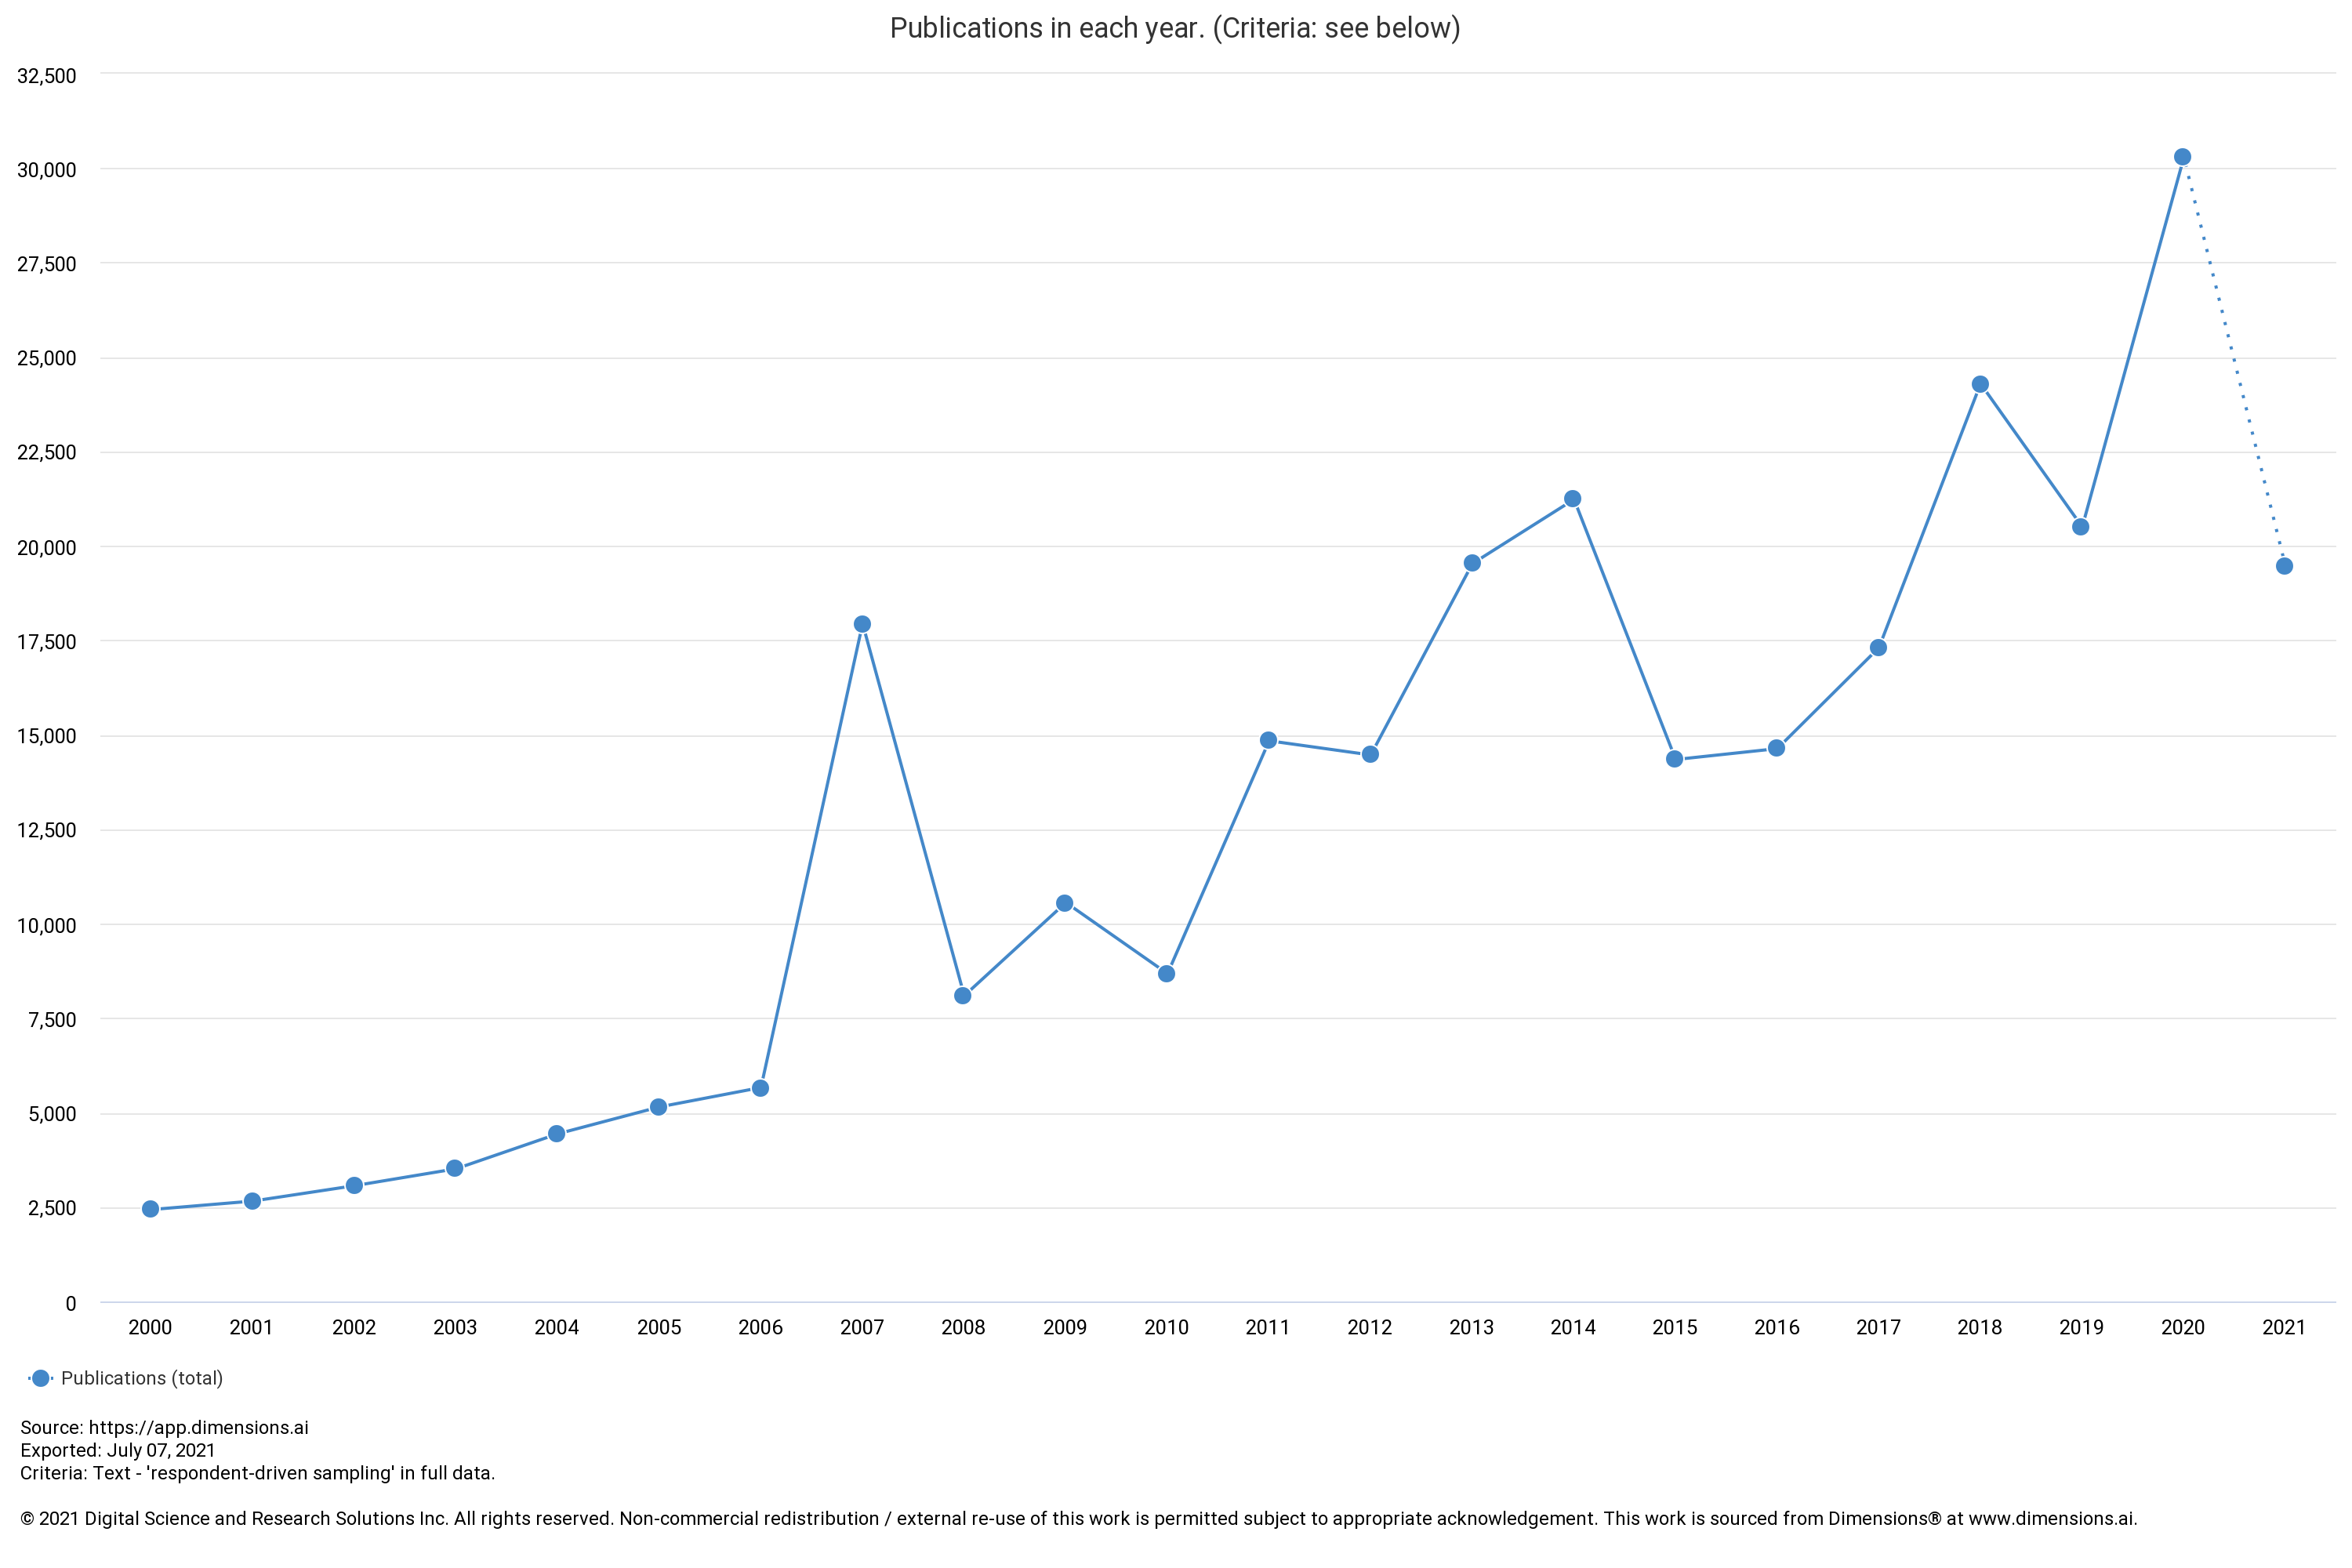
\includegraphics[width=\textwidth]{../../images/rds-yearly-research.png}

\end{frame}

\begin{frame}{Respondent-driven sampling}
  \begin{figure}
    \begin{overprint}
    \onslide<1>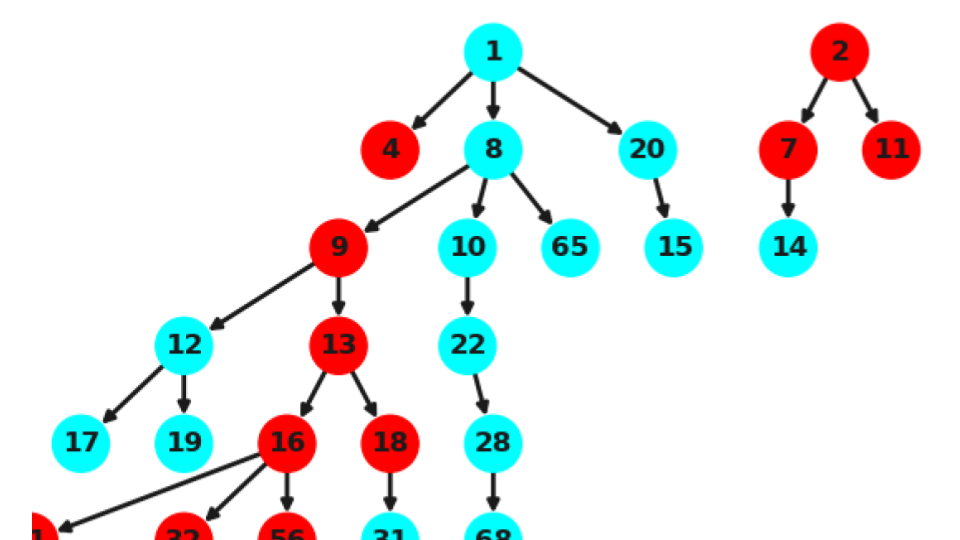
\includegraphics[width=\textwidth]{../../images/graph-rds-harvard-1.png}
    \onslide<2>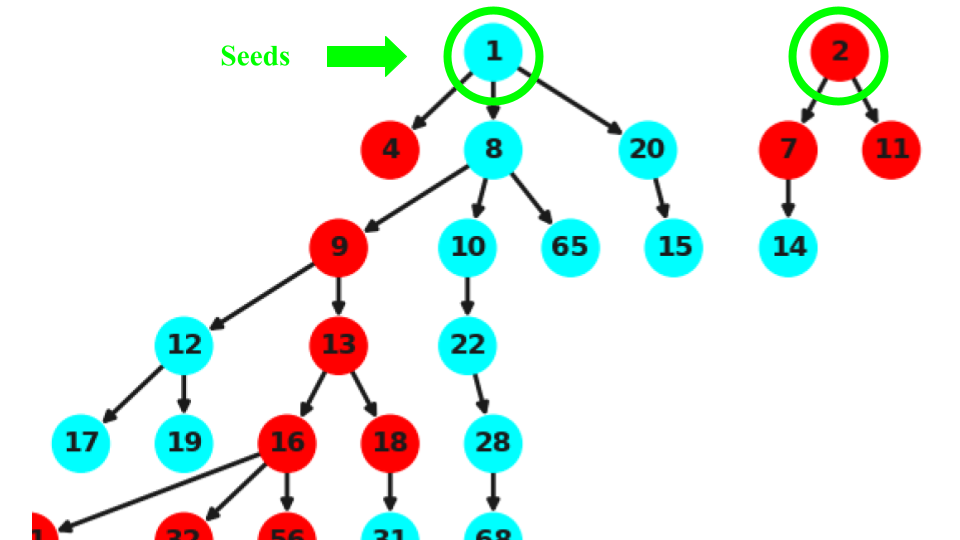
\includegraphics[width=\textwidth]{../../images/graph-rds-harvard-2-english.png}
    \onslide<3>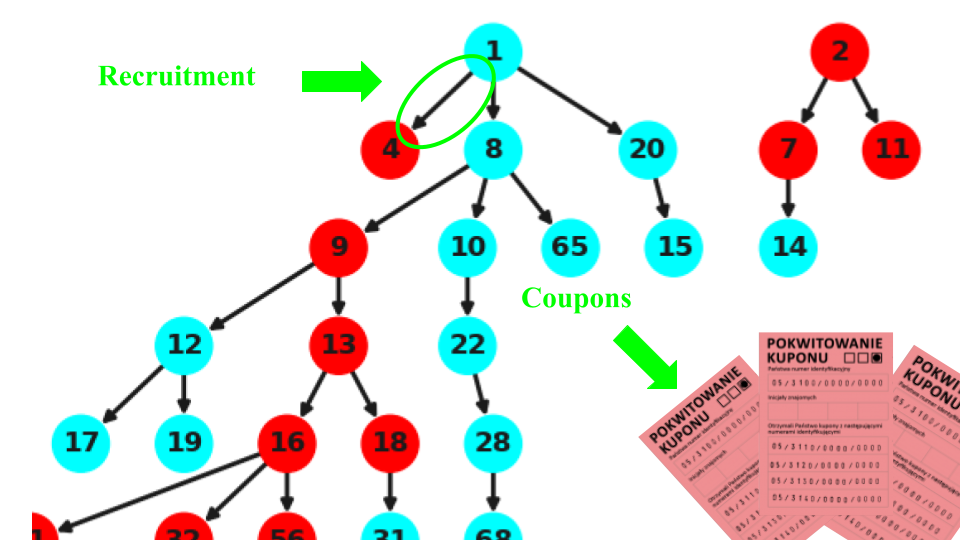
\includegraphics[width=\textwidth]{../../images/graph-rds-harvard-3-english.png}
    \onslide<4>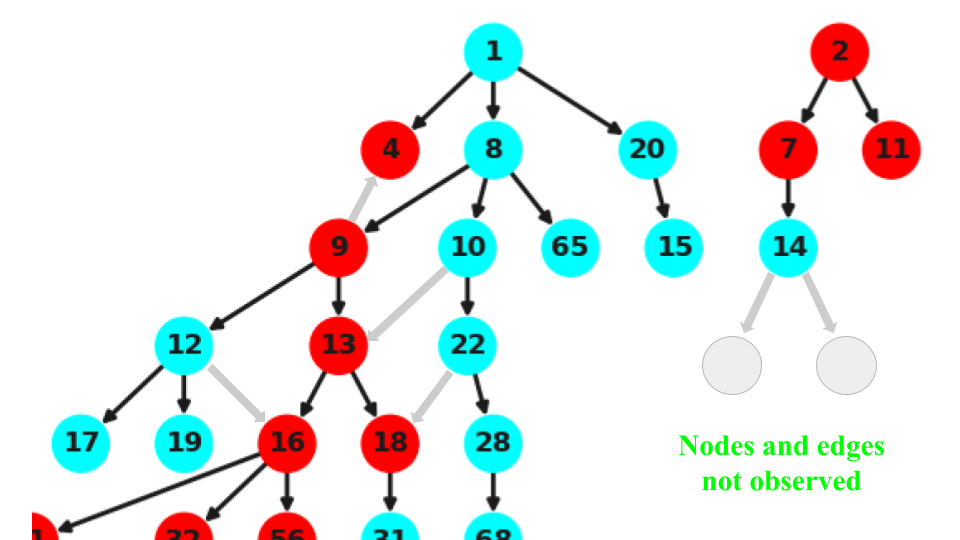
\includegraphics[width=\textwidth]{../../images/graph-rds-harvard-4-english.png}
    \end{overprint}
  \end{figure}  
\end{frame}

\begin{frame}
  
  \frametitle{Dual system of incentives}
    
  Two different sources of theoretical incentive (dual incentive system):

  \Space

  \begin{itemize}
    \justifying
    \item<1> {\bf Individual-sanction based control:} reward for participating
    in the research. 

    \Space

    \item<2> {\bf Group-mediated social control:} reward for recruiting peers.
    When social approval is important, it's more efficient and cheaper.
    Material incentive can be transformed into symbolic incentive . 
  \end{itemize}

\end{frame}

%------------------------------------------------------

\section{Mathematical formulation}

\begin{frame}
  
  \frametitle{Formal model}

  The RDS can be built mathematically with different approaches: 

  \Space

  \begin{itemize}
    \justifying

    \item {\bf Markov process} \cite{heckathorn1997}
  
    Each recruiter's social characteristics affect the characteristics of the
    recruits. There are a limited number of states that subjects can assume and
    the recruits are function of the recruiter characteristics.
  \end{itemize}

  \Space

  \begin{itemize}
    \justifying

    \item {\bf Graphical structure} \cite{crawford2016}
    
    A hidden population is an undirected graph, and we observe it partially in
    the {\em recruitment graph}, as also the coupon matrix and recruitment
    times. The unobserved graph is treated as {\em missing data} and can be
    interpreted as an Exponential Random Graph Model.
  \end{itemize}  

\end{frame}

\subsection{Markov process}

\begin{frame}
  \frametitle{Markov chain model}
  
  \begin{itemize}
    \justifying
    \item In a survey, questions create states describing the participant;
    
    \Space
  
    \item Heckathorn concluded that the recruitment was a memoryless
    process and first-order Markov process.
    
    \Space

    \item The Markov chain indicates the most recent recruit's characteristic;
    
    \Space
  
    \item The Markov chain must be ergodic. 
  \end{itemize}
  
  \end{frame}

\begin{frame}
  
  \frametitle{Markov chain model}

  \begin{figure}
    \begin{overprint}
    \onslide<1>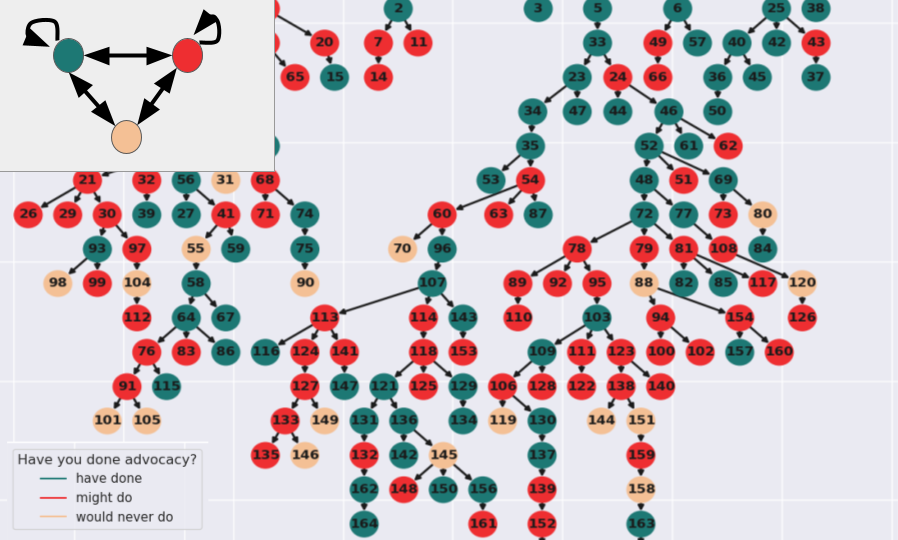
\includegraphics[width=0.98\textwidth]{../../images/rds-markov-harvard-1.png}
    \onslide<2>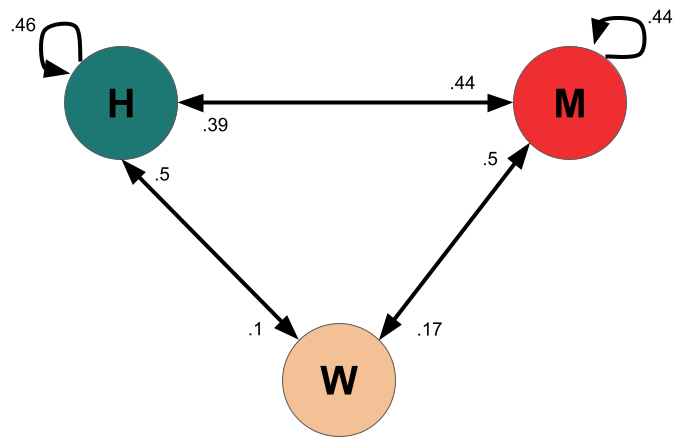
\includegraphics[width=0.98\textwidth]{../../images/rds-markov-harvard-2.png}
    \end{overprint}
  \end{figure}  
  
\end{frame}

\begin{frame}
  \frametitle{Consequences of Markov chain theory}

  \begin{theorem}
    \justifying
    An equilibrium mix of recruits will be attained when the number of waves
    goes to infinity, and it is independent from which recruitment began. The
    pooling approaches the equilibrium in a geometric rate. 
  \end{theorem}

\end{frame}

\begin{frame}
  \frametitle{Convergence analysis}

  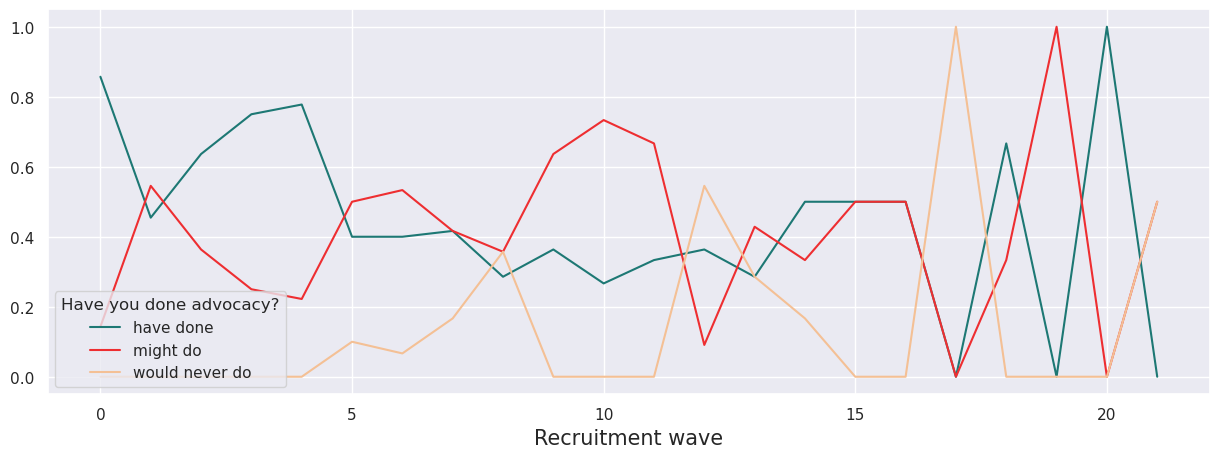
\includegraphics[width=\textwidth]{../../images/recruitment-wave-convergence.png}
\end{frame}

\begin{frame}
  \frametitle{Assessing bias in RDS}

  \begin{itemize}
    \justifying

    \item Inbreeding bias event: there is a positive probability of the subject recruit
  from in-group with certainty. This is also called {\em homophily}.

    \Space 

    \item The paper's conclusion is that RDS produces unbiased samples if the
    inbreeding bias event is equal for all groups.
  \end{itemize}

\end{frame}

\begin{frame}
  \frametitle{Evolution of RDS}

  \begin{enumerate}
    \justifying

    \item<1> \cite{heckathorn2002respondent} extended the model considering symmetric
    relations, that is, is A relates to B, B relates to A. The model was
    called {\em reciprocity model}. Self-reported degrees were also added to
    the model. 

    \item<2> Bootstrap was used to estimate standard deviation of the
    estimations. The ideia is to use the transition matrix to generate a
    Markov chain. \cite{salganik2006variance} improves the variance estimator.
    
    \item<3> Under some regularity conditions, population estimates are
    asymptotically unbiased \cite{salganik2004sampling}.    
    
    \item<4> The RDS II estimator and an analytical variance estimation is
    presented in 2008 \cite{volz2008probability}.
  \end{enumerate}

\end{frame}

\subsection{Graphical structure}

\begin{frame}
  \frametitle{Network model}

  \begin{figure}
    \begin{overprint}
    \onslide<1>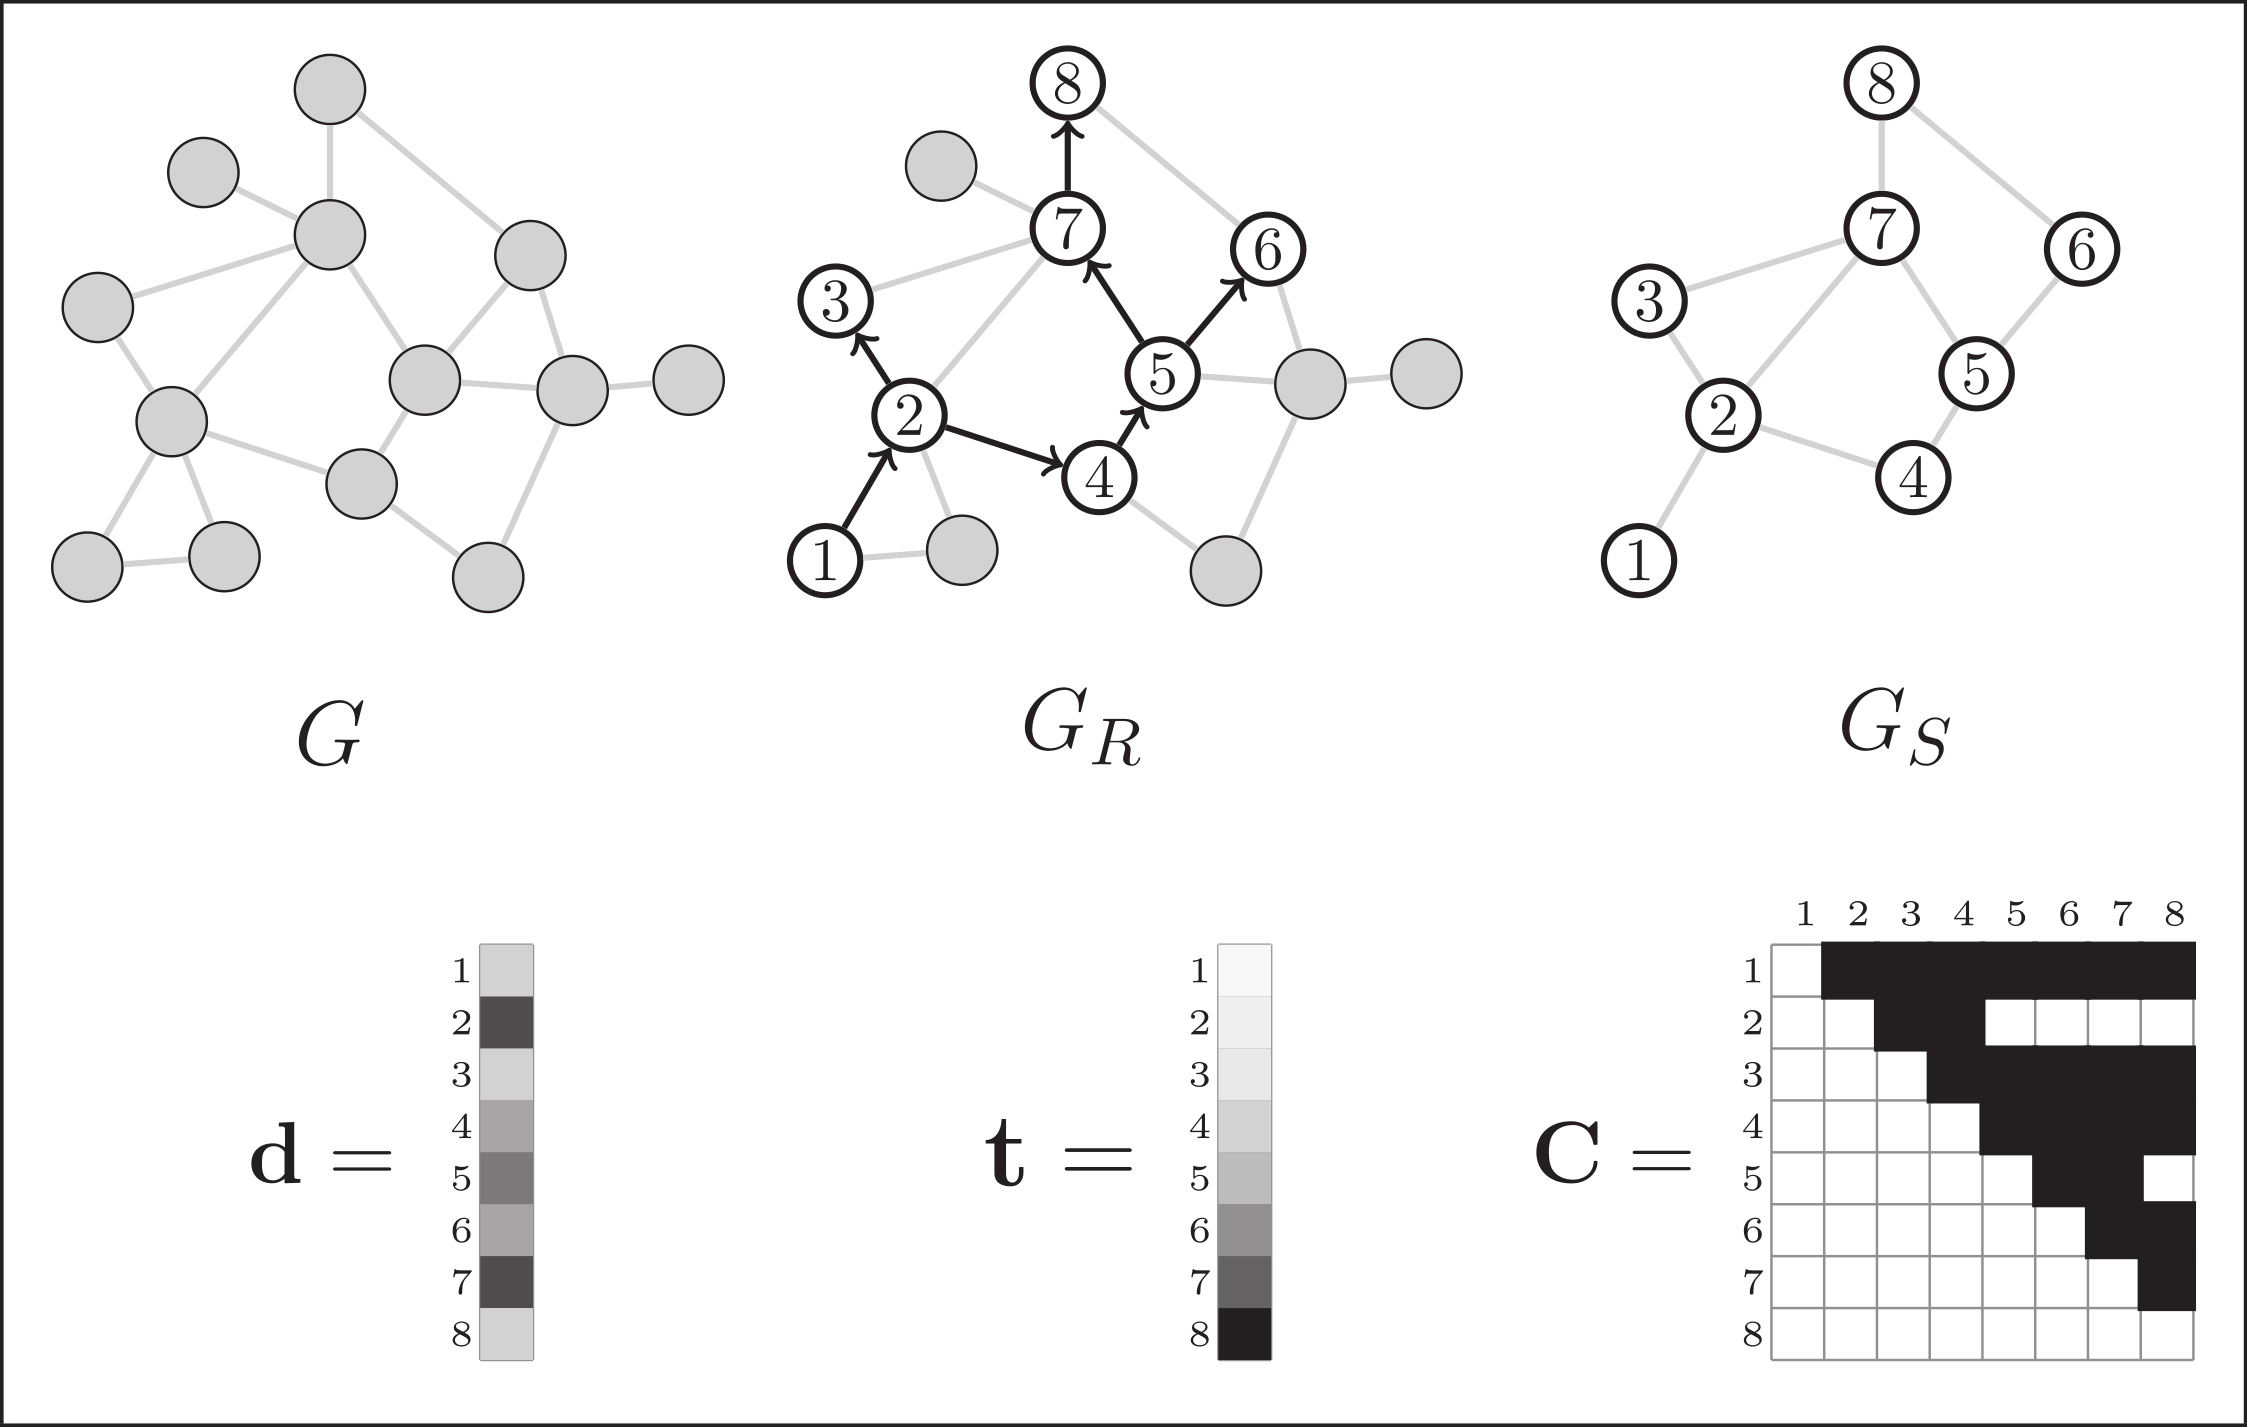
\includegraphics[width=0.98\textwidth]{../../images/graphical-model-example-1.png}
    \onslide<2>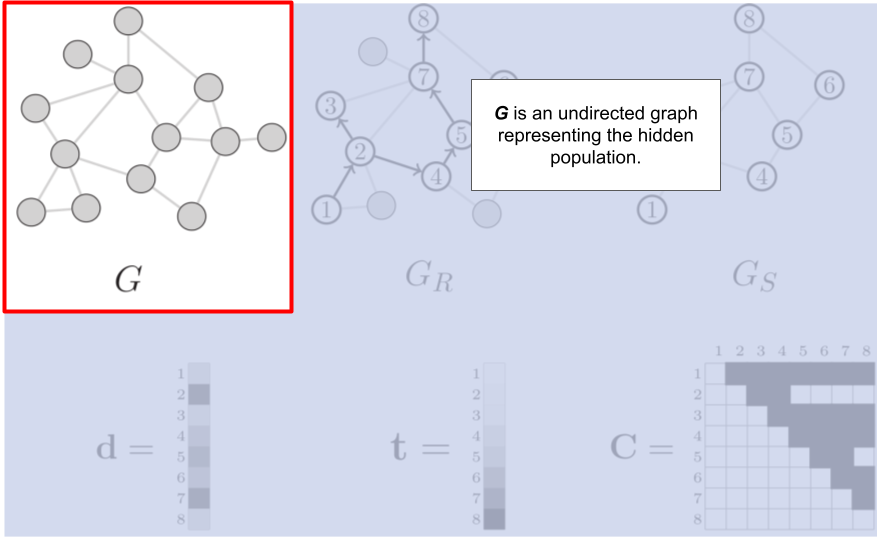
\includegraphics[width=0.98\textwidth]{../../images/graphical-model-example-2.png}
    \onslide<3>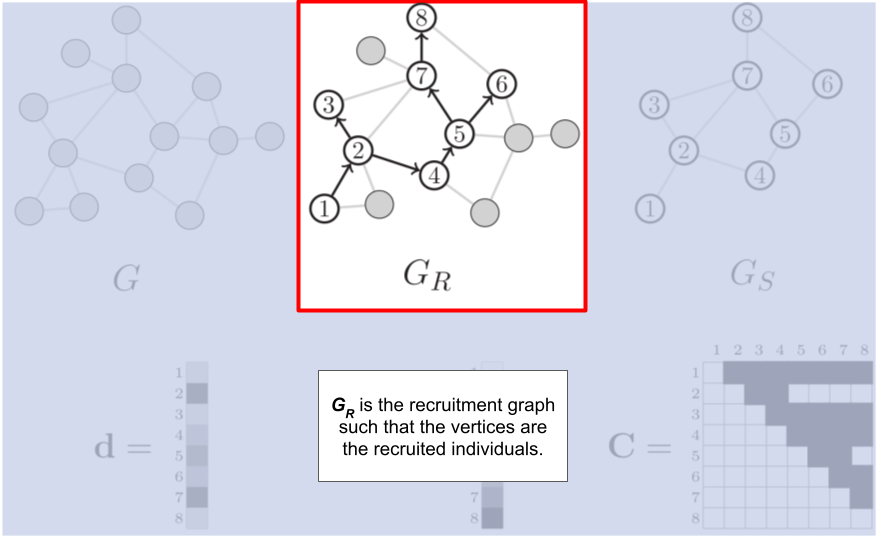
\includegraphics[width=0.98\textwidth]{../../images/graphical-model-example-3.png}
    \onslide<4>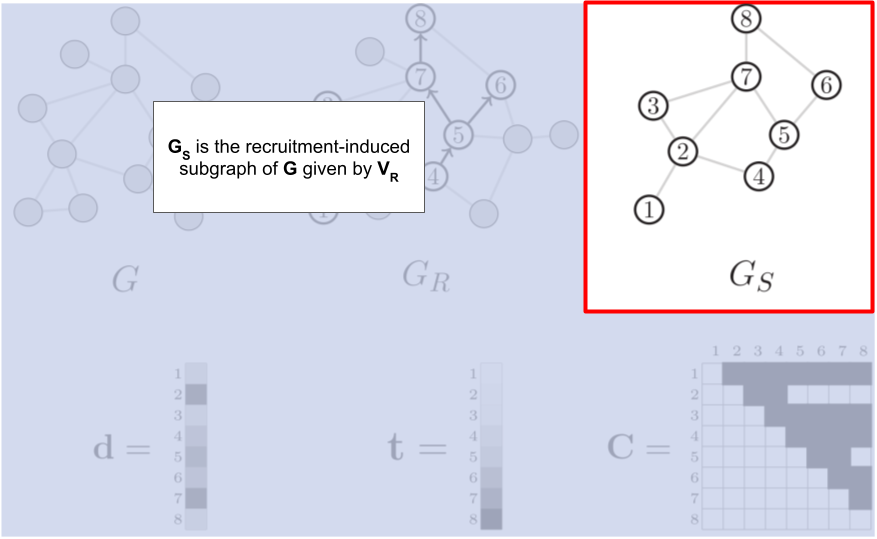
\includegraphics[width=0.98\textwidth]{../../images/graphical-model-example-4.png}
    \onslide<5>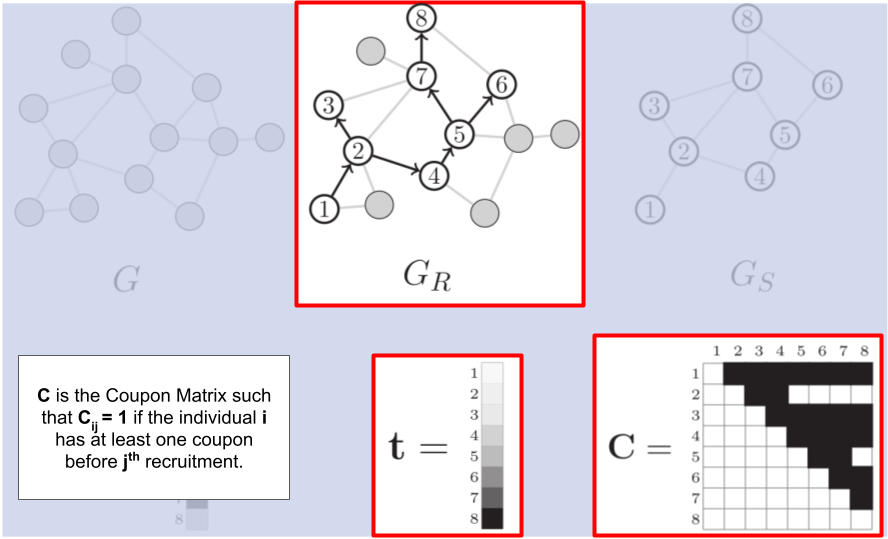
\includegraphics[width=0.98\textwidth]{../../images/graphical-model-example-5.png}
    \onslide<6>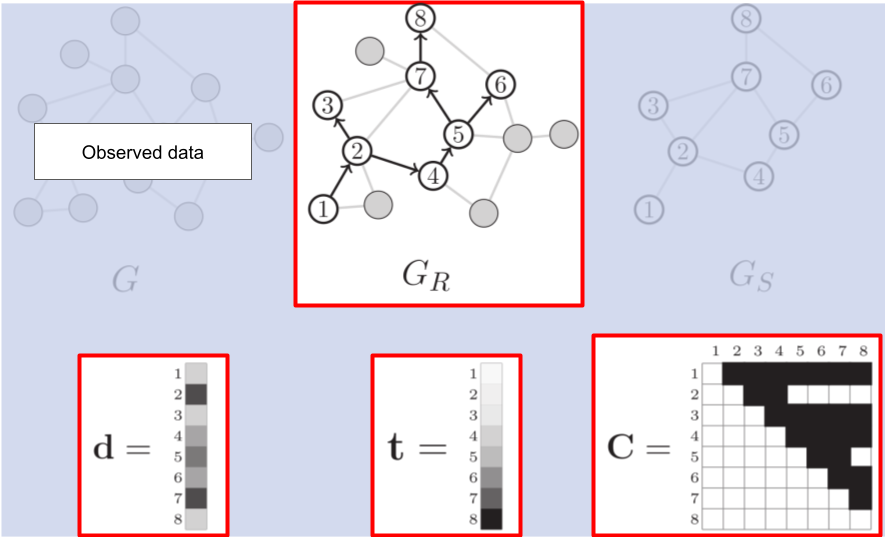
\includegraphics[width=0.98\textwidth]{../../images/graphical-model-example-6.png}
    \end{overprint}
  \end{figure}  
  
\end{frame}

\begin{frame}
  
  \frametitle{Consequences}
  
  \justifying
  The time to recruitment along a {\em susceptible edge} has Exponential
  distribution, independent of the identity, neighbor, and all the other
  waiting times.

  \begin{theorem}[Waiting time for a recruitment]
    \justifying

    Let $u$ be a recruiter and $v \in S_u$ a susceptible neighbor. The waiting
    time to $u$ recruit $v$ conditioned on the recruitment event has
    Exponential distribution with rate $\lambda |S_u|$. The probability of $v
    \in S_u$ to be the next recruited is uniform.  
  \end{theorem}

  \begin{theorem}[Waiting time for some recruitment to occur]
    \justifying

    The waiting time to the next recruitment is distributed as Exponential
    with rate $\lambda \sum_{u \in R} |S_u|$.  
  \end{theorem}

\end{frame}

\begin{frame}
  
  \frametitle{Likelihood of the recruitment time series}

  \begin{block}{Compatibility}
    \justifying

  An estimated subgraph $\hat{G}_S = (\hat{V}_S, \hat{E}_S)$ is {\em
  compatible} with the data if:
  \begin{enumerate}
    \item The vertices in the estimated subgraph are the same as the observed vertices;
    
    \item Each recruitment edge is an undirected edge of the estimated subgraph;
    
    \item For all $v \in V_R, \sum_{u \in V_R / \{v\}} \mathbbm{1}_{\hat{E}_S}(\{u,v\}) \le d_v $.
  \end{enumerate} 
    
  \end{block}

\end{frame}

\begin{frame}
  
  \frametitle{Likelihood of the recruitment time series}

  Let $A$ be the adjacency matrix of a compatible estimated subgraph, that is,
  $$
  [A]_{ij} = 1 \text{ iff } \{i,j\} \in G_S.
  $$
  Then 
  $$
  [AC]_{ij} = \sum_{k} [A]_{ik}[C]_{kj} = \sum_{k} \mathbbm{1}(\{i,k\} \in G_S \text{ and } k \text{ can recruit in } t_j),  
  $$
  that is, the number of recruiters connected to $i$ just before the $j^{th}$
  recruitment, when $j \le i$. Let $u_i$ be the number of edges linking the
  sampled node $i$ with others not sampled. Then, 
  $$
  [C^T u]_{i} = \sum_{k} [C]_{ki} u_k  = \sum_k \mathbbm{1}(k \text{ can recruit in } t_i)\cdot \#\text{susceptible edges of }k 
  $$

\end{frame}

\begin{frame}
  \frametitle{Likelihood of the recruitment time series}

  The likelihood of the recruitment time series $w = (0, t_2 - t_1, ..., t_n -
  t_{n-1})$ is 

  $$
  L(w| G_S, \lambda) = \left(\prod_{k \text{ isn't seed}} \lambda s_k\right) \exp(-\lambda s^Tw), 
  $$
  where 
  $$
  s = \operatorname{tril}(AC)^T 1 + C^Tu 
  $$
  indicates the number of susceptible edges just before each recruitment.

\end{frame}

\begin{frame}
  \frametitle{Likelihood of the recruitment time series}

  Setting $T(A) = -\lambda s$ and $B(A) = \sum_{k \text{ isn't seed}}
  \log(\lambda s_k)$, the likelihood from above can be normalized to obtain
  the probability 
  $$
  P(A|w) \propto \exp\left[T(A)^Tw + B(A)\right]
  $$
  which can be interpreted as an Exponential Random Graph Model. 
\end{frame}

\begin{frame}
  \frametitle{Reconstruction of the recruitment-induced subgraph}

  The ideia is to sample from 
  $$
  p(G_S, \lambda | G_R,C,d,t) \propto L(w|G_S, \lambda) P(G_S)\pi(\lambda), 
  $$
  where $P(G_S)$ and $\pi(\lambda)$ are the prior distributions. For instance,
  it can be taken uniformly over the compatible subgraphs. A
  Metropolis-within-Gibbs sampling scheme is used to draw pairs $(G_S,
  \lambda)$. 

\end{frame}
  
\section{Applications}

\begin{frame}
  \frametitle{Applications}

  \begin{enumerate}
    \item HIV prevalence estimation \cite{gile2011improved}: improved
    RDS II and applied to three different sites.
    
    \Space

    \item Sampling for understanding: Jazz musicians in New York and San
    Francisco. Comparison with data from American Federation of Musicians
    \cite{salganik2004sampling}. 

    \Space
    
    \item Hidden population size estimation \cite{crawford2018hidden}. 
  \end{enumerate}
\end{frame}

\begin{frame}
  \frametitle{Hidden population size estimation}

  \begin{itemize}
    \justifying
    
    \item Let $\mathcal{G}$ be a Erdős-Rényi random graph with probability
    $p$. Then the degree of vertex $i$ is $d_i \sim \operatorname{Bin}(N-1,
    p)$. Assume the hidden population has this distribution. 
    
    \item The probability of recruitment depends only on the edges it shares
    with recruiters. This allows the construction of $L(N,p; G_S, Y)$. 
    
    \item Consider the likelihood of the recruitment time series. 
    
    \item Establishing priors $\pi(N), \pi(p), \pi(G_S), $ and $\pi(\lambda)$.
    Then, the paper obtains the marginal distribution of $N$ given the data
    $$P(N, p|G_S, G_R, C, d, t) \propto L(N, p; G_S, G_R, C, d, t)\pi(N)\pi (p).$$
    
  \end{itemize}

\end{frame}

\begin{frame}
  \frametitle{Hidden population size estimation: algumas conclusões}

  \begin{itemize}
    \justifying
    
    \item Erdos-Rényi model has proven to be empirically useful in a wide
    variety of population size estimation applications; 

    \item RDS was not designed for population size estimation, and it should not be used for this purpose.
    
  \end{itemize}

\end{frame}

\section{Evaluation and critiques}

\begin{frame}
  \frametitle{Evaluation}

  \begin{itemize}
    \justifying

  \item \cite{goel2009respondent} High-homophily breakpoint, when the
  probability of within-group recruitment is high. The convergence requires
  many more waves; 

  \item \cite{mccreesh2012evaluation} concluded that only a third of the RDS
  estimates were closer to the true proportions. The Bootstrap intervals were
  underestimated. This influenced \cite{baraff2016estimating} to improve the
  method;

  \item The estimates validity depends on multiple assumptions that frequently do not hold in the field;
  
  \item \cite{shi2019model} shows how the model can be adjusted to specific
  cases to reduce bias. 
  \end{itemize}

\end{frame}

\begin{frame}[t, allowframebreaks]
   \frametitle{References}
   \bibliographystyle{apalike}
   \bibliography{biblio}
 \end{frame}

\end{document}